\section{The intuition behind SVD}

In this section we will provide several informal ways of looking at
the SVD factorization, aiming to ignite the formal discussion of next
section (where we prove the SVD theorem). \\

\subsection{SVD as a function composition}

The first thing to remember, is that matrices are the operational
representation of an special type of function between vector
spaces\footnote{The reader is invited to review any Linear Algebra
  textbook, to recall the definition of a vector space}
called linear transformations (also called linear mappings or linear
  functions). We say is an operational representation, in the 
sense that they provide an explicit recipe to apply the
function. Furthermore, the functions they represent are
special, as they have the nice property of preserve algebraic
structure across domain and codomains. Such 
property can be summarized as: \\

\[
f(\alpha x + \beta y) = \alpha f(x) + \beta f(y)
\]
\hfill

Where the addition and products mentioned above, are the vector
addition and multiplication by an scalar; defined for vector
spaces. For the specific case of this work, where we restrict
our attention to real matrices, we can tell that they do represent
functions $f: \R{n} \fromto \R{m}$. \\

In this context of linear functions, the matrix multiplication is the
operational representation of the composition of the associated
functions. A matrix factorization is in essence, a way to understand
what the underlying function does; the whole product can be seen as
serial algorithm, where each matrix represents on particular step or
transformation. Each of the four matrices that appear on the SVD
factorization, has its own function as follows:  

\begin{itemize}
\item $A$ is a function $\func{F_A}: \R{n} \fromto \R{m}$
\item $V$ is a function $\func{F_V}: \R{n} \fromto \R{n}$
\item Same goes for  \trans{V}, which is $\func{F_{\trans{V}}}: \R{n} \fromto \R{n}$
\item $\Sigma$ is a function $\func{F_\Sigma}: \R{n} \fromto \R{m}$
\item $U$ is a function $\func{F_U}: \R{m} \fromto \R{m}$
\end{itemize}
\hfill

Thus, in the context of function compositions, the SVD factorization
can be restated as: \\

\[
\func{F_A}(\vec{x}) = \func{F_U}(\func{F_\Sigma}(\func{F_{\trans{V}}}(\vec{x})))
\]
\hfill

\subsection{SVD as a change of basis}

Next thing to remember, are the specially nice properties of orthogonal
matrices. By definition they are square matrices ($n \times n$), and
their columns form an orthonormal basis of \R{n}; this property
implies that they are invertible, but also, that the inverse is
specially easy to compute: it is just the transpose. In addition,
orthogonal matrices are an special case of change of basis matrices:
if $Q$ is an orthogonal matrix, then it can be seen as a function
which takes vectors in the coordinates of its column basis, and that
spits as result the coordinates in the canonical basis. On the same
line, $\inv{Q}$ does represent the opposite change of basis
(from the canonical coordinates to those in terms of the columns of
$Q$). \\

Having set the proper context, let us restate the SVD factorization as
a sequence of successive transformations:

\begin{enumerate}
\item Start with a vector $\vec{x} \in \R{n}$ in canonical coordinates.
\item Perform a change of basis using matrix \trans{V}, from the
  canonical coordinates to those in terms of the columns of $V$.
\item Once expressed as coordinates of columns of $V$, apply the
  linear transformation $\Sigma$; this not only converts the vector
  from \R{n} to \R{m}, but also expresses the coordinates in terms of
  the columns of $U$.
\item Once transformed, perform another change of basis using matrix
  $U$; from the coordinates of columns of $U$ to the canonical ones
  We end then with a vector in \R{m}.
\end{enumerate}
\hfill

\subsection{SVD as a geometrical interpretation}

And what was the advantage of the factorization then? In simple terms,
decomposing the function behind matrix $A$, as a sequence of three
simpler (easier to understand) transformations. Here the geometric
interpretation helps to complete the picture, as orthogonal (change of
basis) matrices do represent rigid transformation in space, that is,
they do not alter the lengths of vectors (hence, preserve
shapes). Strictly speaking, orthogonal matrices can be decomposed as a
rotation and a reflection; but for geometric intuition, is often
desirable to think in the rotation part only. \\

On the other hand, diagonal matrices are the simplest transformation
possible, they do not change the basis but just expand or contract the
coordinates along the axis given by the basis. Again, if we consider
the generic case of diagonal matrices, a negative element $D_{ii}$
would additional provoke a reflection in the axis $i$; but since the
SVD decomposition produces only positive elements on the diagonal, we
ignore this case and just think in terms of contractions or
expansions along the axes. \\

Armed with this geometrical insight, we can enhance our understanding
of the action of $A$ through the SVD decomposition, by associating to
the simpler operations the corresponding geometrical transformations.
The geometric visualization usually requires a couple of
simplifications: first of all, the dimensions of domain and codomain
must be reduced; as it is easier to visualize things in \R{2} or
\R{3}, than in an arbitrary \R{n}. Given two dimensions fit well in a
screen, let us pick $\R{n} = \R{m} = \R{2}$. \\

Secondly, we need to focus our attention in an specific set of
points (as visualizing the effect of a linear transformation against
``all'' vectors in space, even for \R{2}, is a quite abstract and
complex task). The usual procedure is to pick the vectors in the
unitary sphere in \R{2} (which contains in particular the columns of
$V$, as they are unit orthogonal vectors). \\

Let us proceed now: let the matrix $A$ be of
dimensions $2  \times 2$, the matrices $V$ and $U$ be formed
by unit column vectors $\{\vec{v_1},\vec{v_2}\}$ and $\{\vec{u_1},\vec{u_2}\}$,
respectively; and let matrix $\Sigma$ be $diag(\sigma_1,\sigma_2)$
such that $\sigma_1 > \sigma_2 > 0$. We will additionally assume that
$\sigma_1 > 1$ and $\sigma_2 < 1$, in order to allow them represent an
expansion and contraction, respectively. The previously described steps of
the SVD factorization, can be now augmented with the corresponding
geometrical transformations: \\

\begin{enumerate}
\item Start with unit sphere in \R{2}, with the unit vectors \vec{v_1}
  and \vec{v_2} living inside of it. 
\item Action of \trans{V}: Rotate the space such that \vec{v_1} and
  \vec{v_2} become the new orthogonal basis (this transformation
  leaves the shape of the sphere intact).
\item Action of $\Sigma$: Once rotated, the unit sphere is expanded
  in the direction of \vec{v_1} (per $\sigma_1$), and contracted in the
  direction of \vec{v_2} (per $\sigma_2$). 
\item Action of $U$: Once reshaped, the resulting ellipse is taken
  from the basis $\{u_1,u_2\}$ back to the canonical basis (this
  transformation changes the orientation of the ellipse, given that
  is not a symmetric figure; but still it preserves it shape).
\end{enumerate}
\hfill

These steps can be summarized in the following figure \footnote{Which
  was taken from a \href{http://math.stackexchange.com/questions/243811/visualization-of-singular-value-decomposition-of-a-symmetric-matrix}{MathStackExchange phorum post}, we
  could not locate back the original source though.}: \\

\begin{figure}[h]
  \centering
  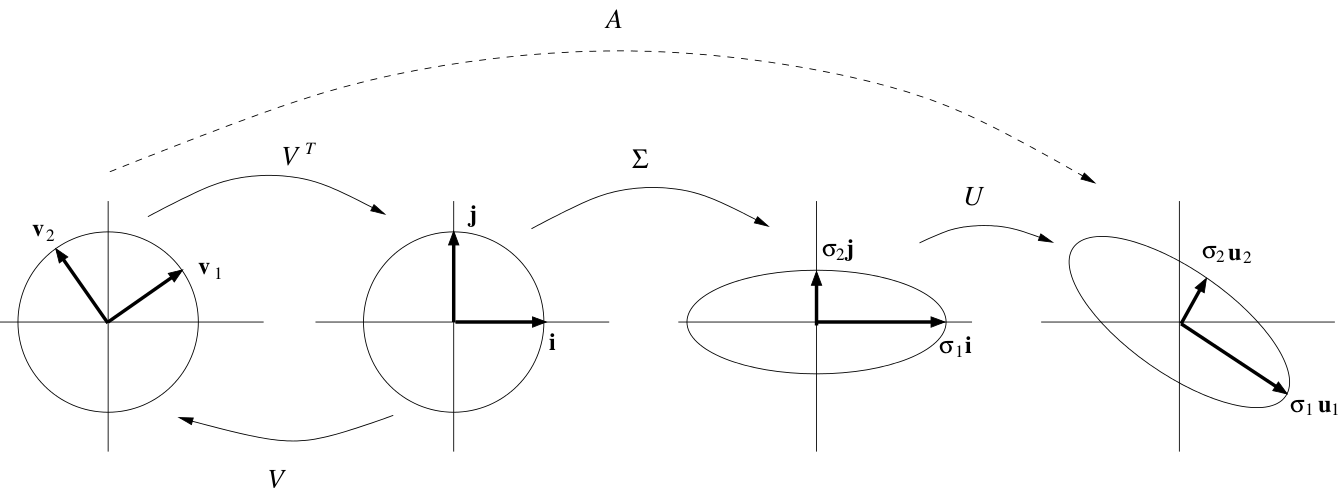
\includegraphics[width=15cm]{svd-geo-diag}
  \caption{Geometrical interpretation of $A = U \Sigma \trans{V}$,
    over the unit sphere.}
  \label{fig:svd-geo-diag}
\end{figure}
\hfill


Although the geometrical interpretation works great for a simple
example in \R{2}, there are a couple of missing details in the action of
matrix $\Sigma$ which are worth mentioning. The first, is that the
dimensions of $\Sigma$ are those of the original matrix ($n \times
m$); therefore, its action is not only expanding or contracting, but
also a migration of space (from \R{n} to \R{m}). If there are more
rows than columns ($m > n$), the transformation $\Sigma$ will produce
a bigger vector than its input (the diagonal entries beyond position
$n$ will be zeroes, which in turn will fill the new vector entries
with zeroes as well; up to $m$ entries). If on the contrary we have
more columns than rows ($m < n$), then the effect will be a truncation
of the input vector (resulting vector has as many entries as rows in
$\Sigma$). In our example, this change of space was not perceived, as $n
= m$. \\

The second omitted detail about the action of $\Sigma$ in 
\cref{fig:svd-geo-diag}, is even more subtle: along with the migration
of space \R{n} to space \R{m}, we are also changing the basis; from
$\{\vec{v_1},\vec{v_2},\dots,\vec{v_n}\}$ to
$\{\vec{u_1},\vec{u_2},\dots,\vec{u_m}\}$. This additional effect may
not be evident at all, but is thanks to an additional property that
is required on the two basis for the SVD factorization to hold:

\[
A\vec{v_i} = \sigma_i\vec{u_i}, \ds{}\forall i=1 \dots r, \ds{}\text{where
} r = rank(A).
\]
\hfill

The above property tells us that the vectors from the two basis were
picked in a very special way: each vector \vec{u_i} is parallel to the
image under $A$ of its associated \vec{v_i}; in other words, the
transformation $A$ maps the \R{n} basis
$\{\vec{v_1},\dots\,\vec{v_n}\}$, into vectors which are parallel to
the \R{m} basis $\{\vec{u_1},\dots\,\vec{u_m}\}$. Given that both basis
are orthonormal, a consequence from this observation is that the
orthogonality of the basis $\{\vec{v_1},\dots\,\vec{v_n}\}$ is preserved
under $A$ (\cite{kalman96}). This is not a trivial property, and not
every basis has it (given $A$ is assumed to be given). This is
actually the key problem of the SVD factorization, and the proofs
provided in the next section, focus around the problem of finding such
special basis.  

